\documentclass[a4paper]{article}

\usepackage{babel}
\usepackage[latin1]{inputenc}
\usepackage{amssymb}
\usepackage{framed}
\usepackage{graphicx}
\usepackage{subcaption}

\setlength{\parindent}{0pt}
\setlength{\parskip}{3ex}

\begin{document}

\begin{center}
  {\large Artificial Neural Networks and Deep Architectures, DD2437}\\
  \vspace{7mm}
  {\huge Short report on lab assignment 3\\[1ex]}
  {\Large Hopfield Networks}\\
  \vspace{8mm}  
  {\Large Rakin Ali, Steinar Logi and Hassan Alzubeidi\\}
  \vspace{4mm}
  {\large February 21, 2024\\}
\end{center}

\section{Main objectives and scope of the assignment}
Our major goals in the assignment were  
\begin{itemize}
\item to build a Hopfield network from scratch only using Python and theory from the lab instructions.
\item to explore associative memory capabilities of a Hopfield network.
\end{itemize}

The weights of the Hopfield network were adjusted to the data points, they were not manually created.

\section{Methods}
All code was created with Python v 3.9 and Jupyter notebook. This assignment was difficult to break into different parts so all instructions were completed three times thereafter we compared our results in order to check if our networks were behaving the way they were suppose to. 

\section{Results and discussion}
This section presents the results provides a small discussion which analyzes the results.

\subsection{Convergence and attractors}
Given x1d, x2d, and x3d where x1d has one bit error while x2d and x3d have two bits errors, we discovered that the network converged towards the stored patterns. When we made the starting pattern even more dissimilar to the stored one where more than half the points were wrong, it did not converge correctly. A result image has been omitted to save space in the report.

\subsection{Sequential update}
All three patterns were stable and tested with the network. The network was able to memorize them. \\
\begin{figure}[htb]
    \centering
    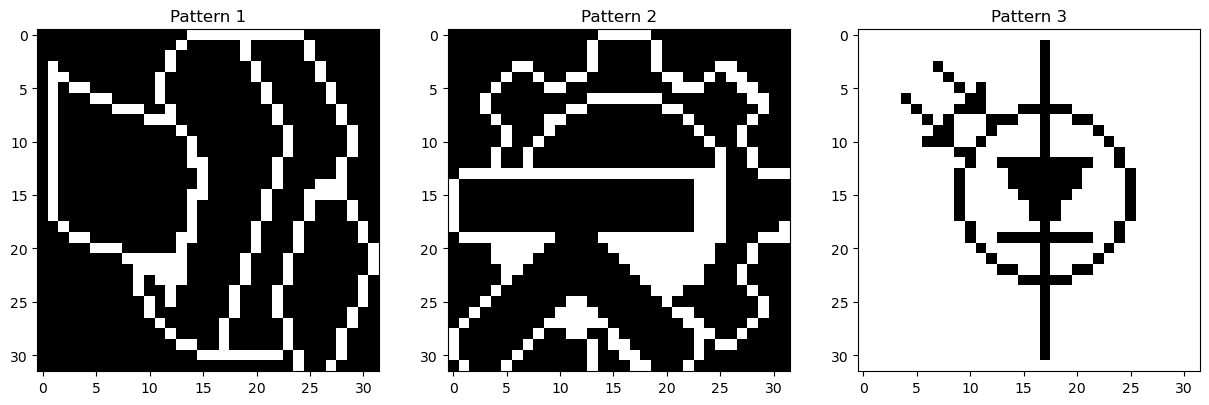
\includegraphics[width=\textwidth]{Labs/Lab 3/Rakin/Results/3.2-3Patterns.png}
    \caption{P1, P2 and P3 recreated with Hopfield network }
    \label{fig:enter-label}
\end{figure}
\\Later when the network tried patterns p10 and p11, interesting results were noted. P10 was handled well while P11 did not. P11 seems to be spurious. See the figure below\\

\begin{figure}[htb]
    \centering
    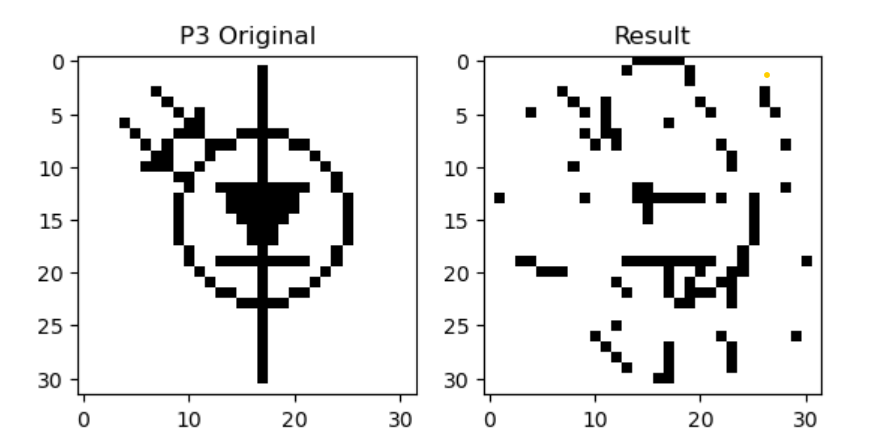
\includegraphics[width=10cm]{Labs/Lab 3/Rakin/Results/3.2-p11.png}
    \caption{P3 on the left and P11 recall on the right}
    \label{fig:enter-label}
\end{figure}

\subsection{Energy}
The energy of a Hopfield network  with relation to the given activations is defined as the following:
$$
E = -\sum_i\sum_j w_{ij}x_ix_j
$$
The energy of the network is guaranteed to decrease after each update if the weights between to nodes in the Hopfield network are symmetric. We initialized the weights using the Hebbian learning rule. We used the first three images in the image dataset and let the network memorize them. The energies at the different images are; -490287 for image 1, -465114 for image 2, and -498090.6 for image 3. We used image 11 from the dataset which is a mix of images 2 and 3. The network's energy when presented with image 11 was around -58197, which is much higher than for the images the network remembered. We performed recall on this image sequentially and plotted the energy after each iteration. The results from that can be seen in figure \ref{fig:energies}

\begin{figure}[ht]
    \centering
    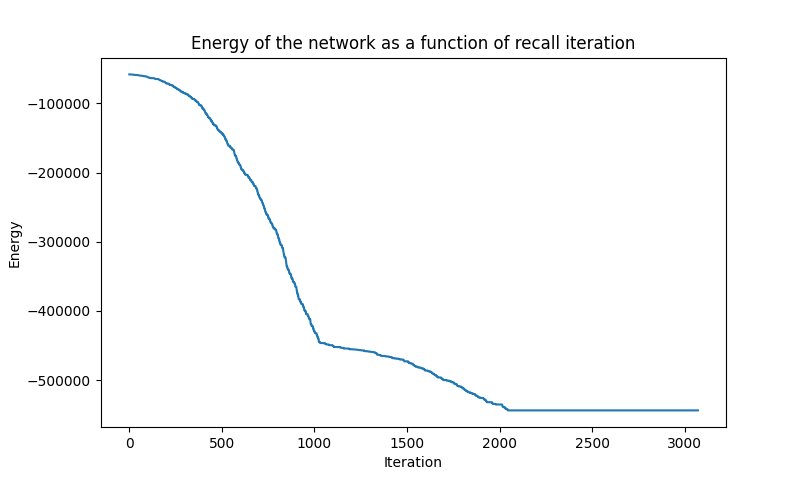
\includegraphics[width=0.8\textwidth]{Labs/Lab 3/images/energy.png}
    \caption{Energy of the network}
    \label{fig:energies}
\end{figure}

As can be seen in figure \ref{fig:energies} the energy either lowers or stays the same after each iteration. This was expected since as mentioned in the beginning of this section one should expect the energy of the network to get lower if the weights are symmetric. We also tried initializing the weights randomly in two ways. One way was initializing each weight using a normal distribution with mean 0 and variance 1 and the other way we used a normal distribution with mean 0 and variance 1 to initialize the weights but we ensured that the weight matrix was symmetrical. Figure \ref{fig:energies-random-weights} shows the evolution of the energy of the network for each iteration when recalling image 11 from the data set.

\begin{figure}[!htb]
    \centering
    \begin{subfigure}[b]{0.48\textwidth}
        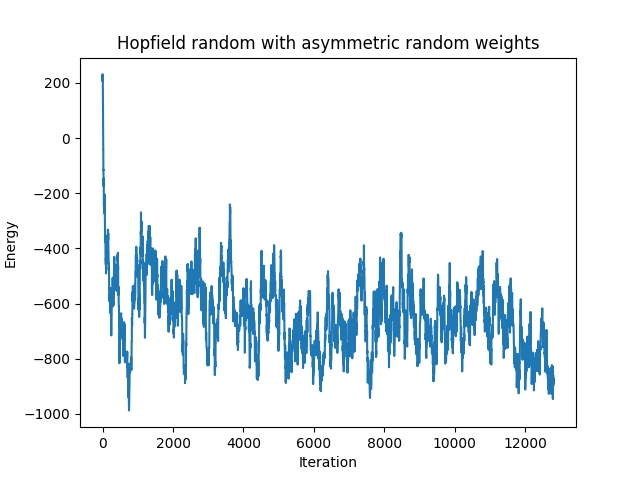
\includegraphics[width=\textwidth]{Labs/Lab 3/images/energies-asymmetric.png}
        \caption{Asymmetric weights}
    \end{subfigure}%
    \hfill
    \begin{subfigure}[b]{0.48\textwidth}
        \centering
        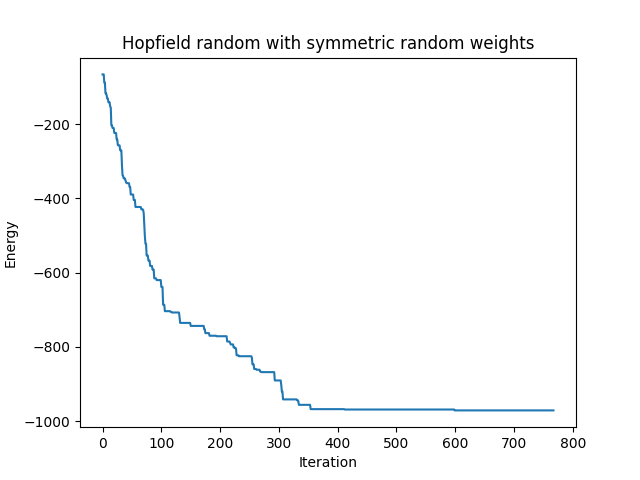
\includegraphics[width=\textwidth]{Labs/Lab 3/images/energies-symmetric.png}
        \caption{Symmetric weights}
        \label{fig:symmetric}
    \end{subfigure}
    \caption{The energy of networks with random weights}
    \label{fig:energies-random-weights}
\end{figure}

As the figure shows the energy of the network with asymmetric weights does not always lower with each iteration, however, the network with the symmetric random weights does lower the energy with each iteration in the recall. It did not recall one of the pictures in the data set, since the network has not memorized the patterns, but it did end in some spurious pattern.

\subsection{Distortion Resistance}
We trained a Hopfield network using images 1, 2 and 3 from the data set. We then distorted the patterns by flipping a random part of the bits. We checked with different levels of distortion, the values we checked were on the interval 0\% to 100\% distortion with a step size of 10\%. The plot in figure \ref{fig:distortions} shows whether we managed to recover the figure using the model as a function of the distortion. The model performed pretty well. It managed to recover the image with up to 40\% distortion. After that, it did not manage to recover the original pattern. However, we noticed that when the percentage of distorted pixels was greater than 50\% it sometimes converged to a pattern that was the original pattern with flipped bits. That is every 1 was flipped to -1 and vice versa. These results can be seen in figure \ref{fig:distortion}. These results are expected since the Hopfield network is symmetric in this way.

\begin{figure}
    \centering
    \begin{subfigure}[b]{0.48\textwidth}
        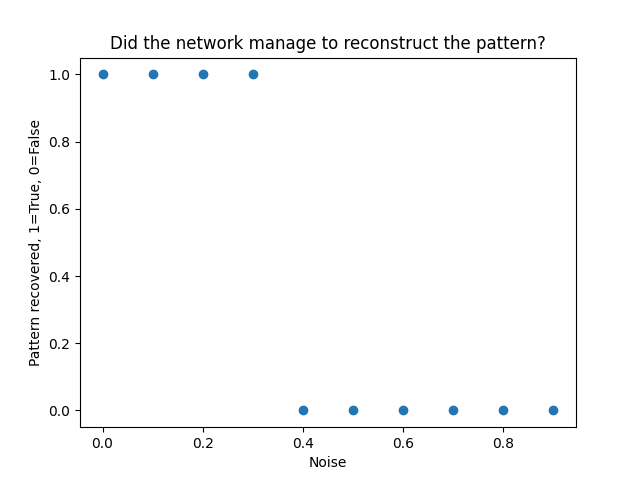
\includegraphics[width=\textwidth]{Labs/Lab 3/images/distortion.png}
    \end{subfigure}
    \hfill
    \begin{subfigure}[b]{0.48\textwidth}
        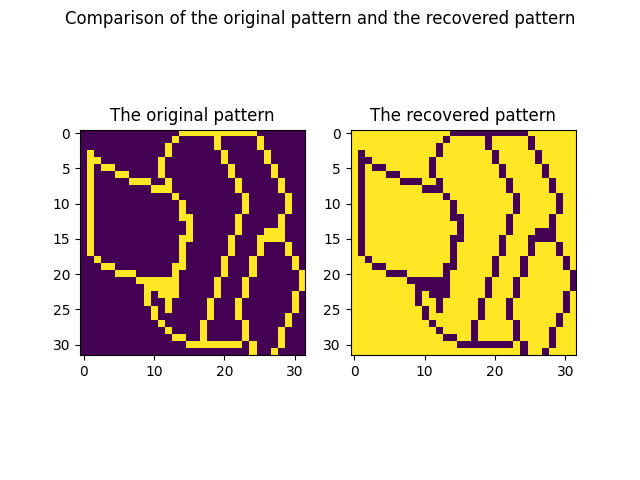
\includegraphics[width=\textwidth]{Labs/Lab 3/images/inverted_pattern.png}
    \end{subfigure}
    \caption{Recovering distorted images}
    \label{fig:distortions}
\end{figure}

\subsection{Capacity}
We compared how many patterns the network can store in two cases. The comparison between pictures and random patterns.
Our results indicate that the network can only store three pictures but store more than three random patterns. We think it's due to the similarity between the random patterns. 

Furthermore, we created a network that consists of 100 nodes to compare how many of the earlier patterns the network can remember once we add more patterns to it. Figure \ref{fig:earlier-patterns}  shows the comparison with and without noise.   



\begin{figure}[ht]
    \centering
    \begin{subfigure}[b]{0.48\textwidth}
        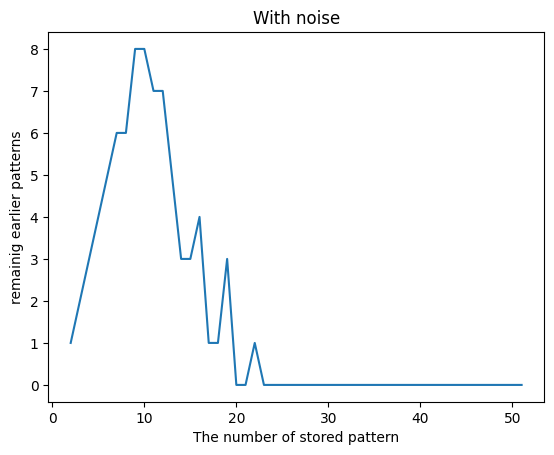
\includegraphics[width=\textwidth]{Labs/Lab 3/Hasan_3/Result_fig/noise.png}
        \caption{Stored patterns with 10\% noise}
    \end{subfigure}
    \hfill
    \begin{subfigure}[b]{0.48\textwidth}
        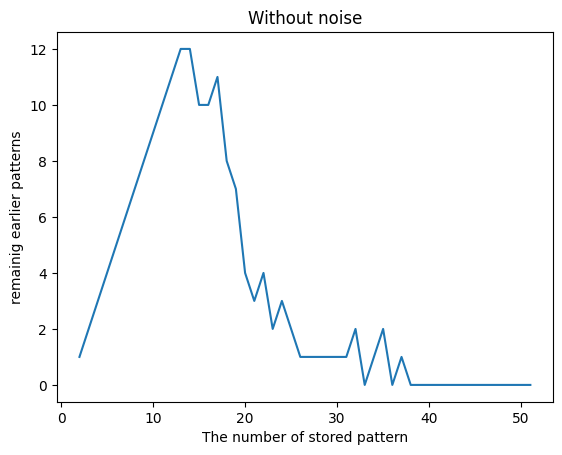
\includegraphics[width=\textwidth]{Labs/Lab 3/Hasan_3/Result_fig/without-noise.png}
        \caption{Stored patterns without noise}
    \end{subfigure}
    \caption{Number of patterns the network was able to store}
    \label{fig:earlier-patterns}
\end{figure}
\subsection{Sparse Patterns}
In this section of the assignment we investigated sparse patterns and how the learning rule could be adjusted using average activity $\rho=\frac{1}{NP}\sum_\mu \sum_i x_i^\mu$. The learning rule with this average activity is:
$$
w_{ij} = \sum_{\mu=1}^P (x_i^\mu - \rho)(x_j^\mu - \rho)
$$

And when we updated the activations during recall we used the following equation that relies on a bias term, $\theta$:

$$
x_i \leftarrow 0.5 + 0.5 * sign(\sum_j w_{ij}x_j - \theta)
$$

We generated patterns with 10\% activity and investigated how many patterns could be stored for different values of the bias term, $\theta$. We checked for values of theta between -3 and 10 and used a step size of 0.1, based on our empirical findings. We made a script that repeated this 100 times and used the average number of patterns stored to get better results. We then plotted the average number of patterns the network was able to store as a function of the theta value. This graph can be seen in figure \ref{fig:stored-patterns-theta}. We also tried this for random patterns with 5\% activity. The results for that can be seen in the graph on the right in figure \ref{fig:stored-patterns-theta}

\begin{figure}[ht]
    \centering
    \begin{subfigure}[b]{0.48\textwidth}
        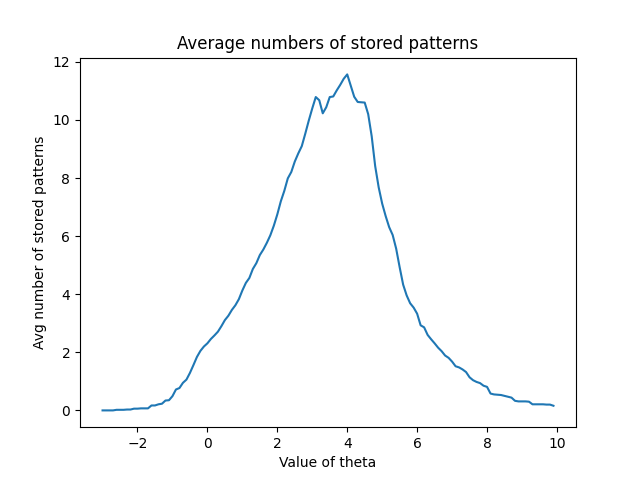
\includegraphics[width=\textwidth]{Labs/Lab 3/images/stored_patterns_theta.png}
        \caption{Patterns with 10\% activation}
    \end{subfigure}
    \hfill
    \begin{subfigure}[b]{0.48\textwidth}
        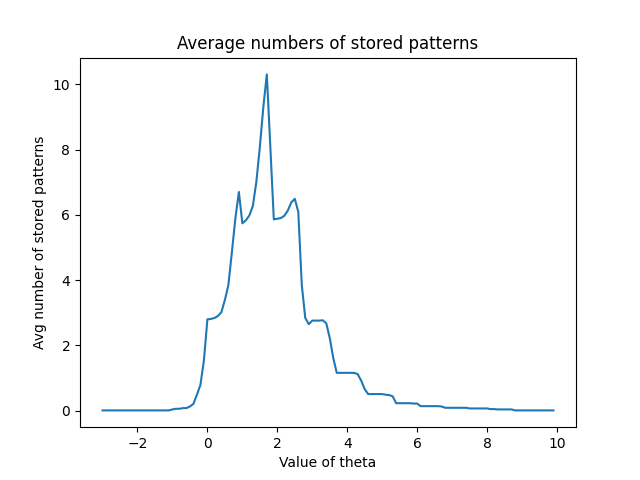
\includegraphics[width=\textwidth]{Labs/Lab 3/images/stored_patterns_theta_005_activity.png}
        \caption{Patterns with 5\% activation}
    \end{subfigure}
    \caption{Number of patterns the network was able to store}
    \label{fig:stored-patterns-theta}
\end{figure}

The network was able to store up to around 12 patterns when the patterns contained 10\% activity with a value of $\theta$ around 3.9. When the activations of the patterns were 5\% the network was able to store up to around 10 patterns using a value of $\theta$ around 2. 


\section{Final remarks}
In this lab we learned that 
\begin{itemize}
    \item Hopfield networks are good at solving optimization problem. By encoding a problem as an energy landscape where each state represents a possible solution and the energy corresponds to the objective function, the network can converge to low-energy states which correspond to optimal solutions. This was learned from section 3.3 
    \item Hopfield networks are used to store patterns and retrieve them based on partial or noisy inputs. They are suitable for tasks such as auto-association and content-addressable memory. This was learned from 3.4 and 3.1 
    \item We learned about the Catastrophic forget phenomenon in Hopfield networks. The network, according to the theory covered in the lecture, can recall roughly 138 patterns from 1000 nodes and once that threshold is exceeded, the network forgets almost everything entirely in an abrupt manner.
    \end{itemize}

\end{document}
